\thispagestyle{fancy}

\begin{appendices}

\chapter{Derivations}
\label{ax:derivations}

\section*{Investment Optimization in Tullock Contests}

A player $i$ wants to find the $I^*$ that maximizes his or her expected profit as expressed in the maximization problem:


\begin{equation}
    \underset{I_i}{\text{max}}\quad\mathbb{E}\Pi_i(I_i,I_j) = \frac{I_i}{I_i + \sum_{j\neq i}^n I_{j}}\mathbb{V} - I_i
\label{eq:exp_util_anex}
\end{equation}

Here, $n$ is the  number of participants in the game.\\
Let us assume that the valuation of the game $\mathbb{V}$ is equal for all players and hence, that the optimal investment $I^{*}$ is equal for everyone. At the maximum of function \ref{eq:exp_util_anex} holds:
\begin{flalign*}
    \frac{d}{dI_i}(\frac{I_i\mathbb{V}}{I_i + \sum_{j\neq i}^n I_{j}} - I_i) = 0 &&
\end{flalign*}
which after deriving using the quotient rule results in:
\begin{flalign*}
    \frac{\mathbb{V}(I_i + \sum_{j\neq i}^n I_{j})-I_i\mathbb{V}}{(I_i + \sum_{j\neq i}^n I_{j})^2}-1&&
\end{flalign*}
Since we know that at the maximum $I_i^{*}=I_{-i}^{*}=I^{*}$ holds, we can simplify:
\begin{flalign*}
    \frac{n\mathbb{V}I^*-\mathbb{V}I^*}{(nI^*)^2}-1 = 0&&
\end{flalign*}
We further simplify to:
\begin{flalign*}
    \frac{\mathbb{V}\bcancel{I^*}(n-1)}{n^2I^{\bcancel{*2}}} = 1&&
\end{flalign*}
Which gives equation \ref{eq:opt_last}:
\begin{flalign*}
    I^{*} = \frac{n-1}{n^2}\mathbb{V}
\end{flalign*}

\section*{Asymmetric Valuations}

An important conundrum that the approach presented in this thesis makes easier to solve than Koch's proposal \cite{koch2017} is a possible difference in valuation of the prize in terms of higher wage since participants with higher ability or higher utility from consumption will profit more from it. \cite{nti1999} shows that in the two player case:\\

\begin{quote}
    "The player who values the prize more expends more effort in equilibrium but both players allocate the same fraction of their valuations to the contest".\footnote{\citet[p.~419]{nti1999}.}
\end{quote}

To show this, we just need to write the FOC for the two players explicitly:\footnote{See Appendix \ref{ax:derivations} for a derivation of the FOC.}

\begin{equation*}
\begin{split}
    \frac{I_j}{(I_j + I_i)^2}\mathbb{V}_i-1 = 0 \\
    \frac{I_i}{(I_j + I_i)^2}\mathbb{V}_j-1 = 0
\end{split}
\end{equation*}

By equalizing we obtain:
\begin{equation}
    \frac{I_i}{\mathbb{V}_i} = \frac{I_j}{\mathbb{V}_j} 
\end{equation}

Now let us consider the case of $n=3$ for $i \in (a,b,c)$ with exactly one winner.\footnote{\cite{stein2002} offers a general derivation for N players.} Using the same process as above we obtain the equation system:

\begin{align}
    \frac{(I_a+I_b)}{(I_a+I_b+I_c)^2}\mathbb{V}_c&=1\\
    \frac{(I_a+I_c)}{(I_a+I_b+I_c)^2}\mathbb{V}_b&=1\\
    \frac{(I_b+I_c)}{(I_a+I_b+I_c)^2}\mathbb{V}_a&=1
\end{align}

To more easily visualize the results, we assume w.l.o.g that $I_a = I$, $I_b = \beta_b I$ and $ I_c = \beta_c I $, and that $\mathbb{V}_a = \mathbb{V}$, $\mathbb{V}_b = \alpha_b \mathbb{V} $ and $\mathbb{V}_c = \alpha_c \mathbb{V}$. The equation system thus is simplified to:

\begin{align}
    \label{eq:sys1}\frac{(1+\beta_b)}{(1+\beta_b+ \beta_c )^2}\alpha_c\mathbb{V}&=I\\
    \label{eq:sys2}\frac{(1+\beta_c )}{(1+\beta_b  + \beta_c )^2}\alpha_b\mathbb{V}&=I\\
    \label{eq:sys3}\frac{(\beta_b +\beta_c )}{(1+\beta_b  + \beta_c )^2}\mathbb{V}&=I
\end{align}

After setting (\ref{eq:sys2}) = (\ref{eq:sys3}) we obtain:

\begin{equation}
    \label{eq:betab}\beta_b=(1+\beta_c)\alpha_b-\beta_c
\end{equation}

Similarly, we set (\ref{eq:sys1}) = (\ref{eq:sys3}) and obtain $(1+\beta_b)\alpha_c=\beta_b+\beta_c$ in which we can replace $\beta_b$ by (\ref{eq:betab}). Solving for $\beta_c$ we get:
\begin{equation}
\label{eq:betac}
    \beta_c = \frac{\alpha_b-\alpha_c-\alpha_b\alpha_c}{\alpha_b\alpha_c-\alpha_c-\alpha_b}
\end{equation}
Which inserted back in (\ref{eq:betab}) gives us:
\begin{equation}
\label{eq:betab2}
    \beta_b=\alpha_b + \alpha_b\frac{\alpha_b-\alpha_c-\alpha_b\alpha_c}{\alpha_b\alpha_c-\alpha_c-\alpha_b}-\frac{\alpha_b-\alpha_c-\alpha_b\alpha_c}{\alpha_b\alpha_c-\alpha_c-\alpha_b}
\end{equation}

Finally, from (\ref{eq:betab2}) and (\ref{eq:betac}) we know that $\beta_b+\beta_c = 1+\alpha_b\frac{\alpha_b-\alpha_c-\alpha_b\alpha_c}{\alpha_b\alpha_c-\alpha_c-\alpha_b}$ and we can replace in \ref{eq:sys3} to obtain:

\begin{equation}
\label{eq:InvDiffVal}
    I = \frac{\alpha_b+\alpha_b\frac{\alpha_b-\alpha_c-\alpha_b\alpha_c}{\alpha_b\alpha_c-\alpha_c-\alpha_b}}{(1+\alpha_b
    +\alpha_b\frac{\alpha_b-\alpha_c-\alpha_b\alpha_c}{\alpha_b\alpha_c-\alpha_c-\alpha_b})^2}\mathbb{V}
\end{equation}

\hfill \break

Now, to more easily see how this function behaves let us assume that only participant \textit{c} has a different valuation and therefore $\alpha_b = 1$. It follows:

\begin{equation}
    I_a=I_c=\frac{2\alpha_c}{(1+2\alpha_c)^2}\mathbb{V}
\end{equation}

The denominator will grow faster for increasing $\alpha_c$ which means that $I_a$ will tend to $0$.\\


The general case is more cumbersome but we can still find some conditions for the relationship between $\alpha_b$ and $\alpha_c$. Requiring that $\alpha_b, \alpha_c \in \mathbb{R}^+$ and that $\alpha_b\alpha_c-\alpha_c-\alpha_b \neq 0$, it can be shown that, in order for $I\geq0$, then $\alpha_b\alpha_c>\alpha_c+\alpha_b$.\\

This means, in particular, that there are some levels for which an investment is no longer profitable, take for instance $\alpha_b = 2$ and $\alpha_c = 4$.\\

A look at the function graph \ref{fig:invest_func} gives us a better understanding of its behavior. For very low levels of others' valuations the investment value is close to zero but increases with $\alpha_b$ and $\alpha_c$. After achieving a maximum of $\frac{1}{4}$, or the equivalent to the two player game, the function decreases monotonically.

\begin{figure}[H]
    \centering
    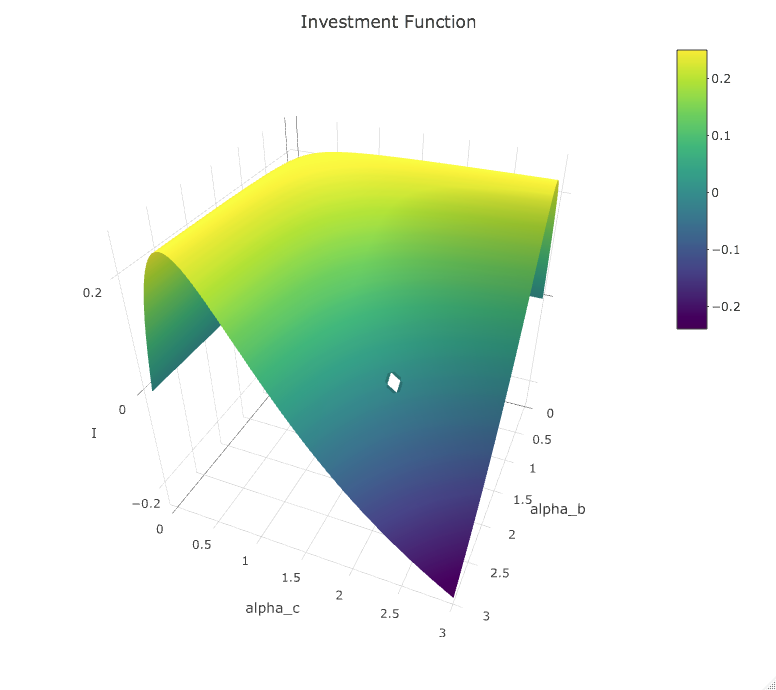
\includegraphics[scale=0.5]{graphs/Investment_Func.png}
    \caption{Investment function dependant on the share of others' valuation}
    \label{fig:invest_func}
\end{figure}

\chapter{Tables}

\begin{table}[!htbp] \centering
\begin{tabular}{@{\extracolsep{5pt}}lcc} 
\multicolumn{3}{l}{Wilcoxon rank sum test with continuity correction}\\
\\[-1.8ex]\hline 
\hline \\[-1.8ex] 
\multicolumn{1}{l}{Piece Rate} & \multicolumn{1}{c}{Statistic} & \multicolumn{1}{c}{p-value}\\
\hline \\[-1.8ex]
High & 1186.5 & 0.8006\\
Low & 1070 & 0.5462\\
\hline \\[-1.8ex] 
\hline \\[-1.8ex]
\multicolumn{3}{l}{\footnotesize{Null Hypothesis: Difference in production between treatments is equal to 0}}\\[2ex]
\end{tabular}
  \caption{Comparison of productions in the benchmarking rounds between treated and non-treated groups} 
  \label{tab:bench_prods_test} 
\end{table} 


    \begin{figure}
        \centering
        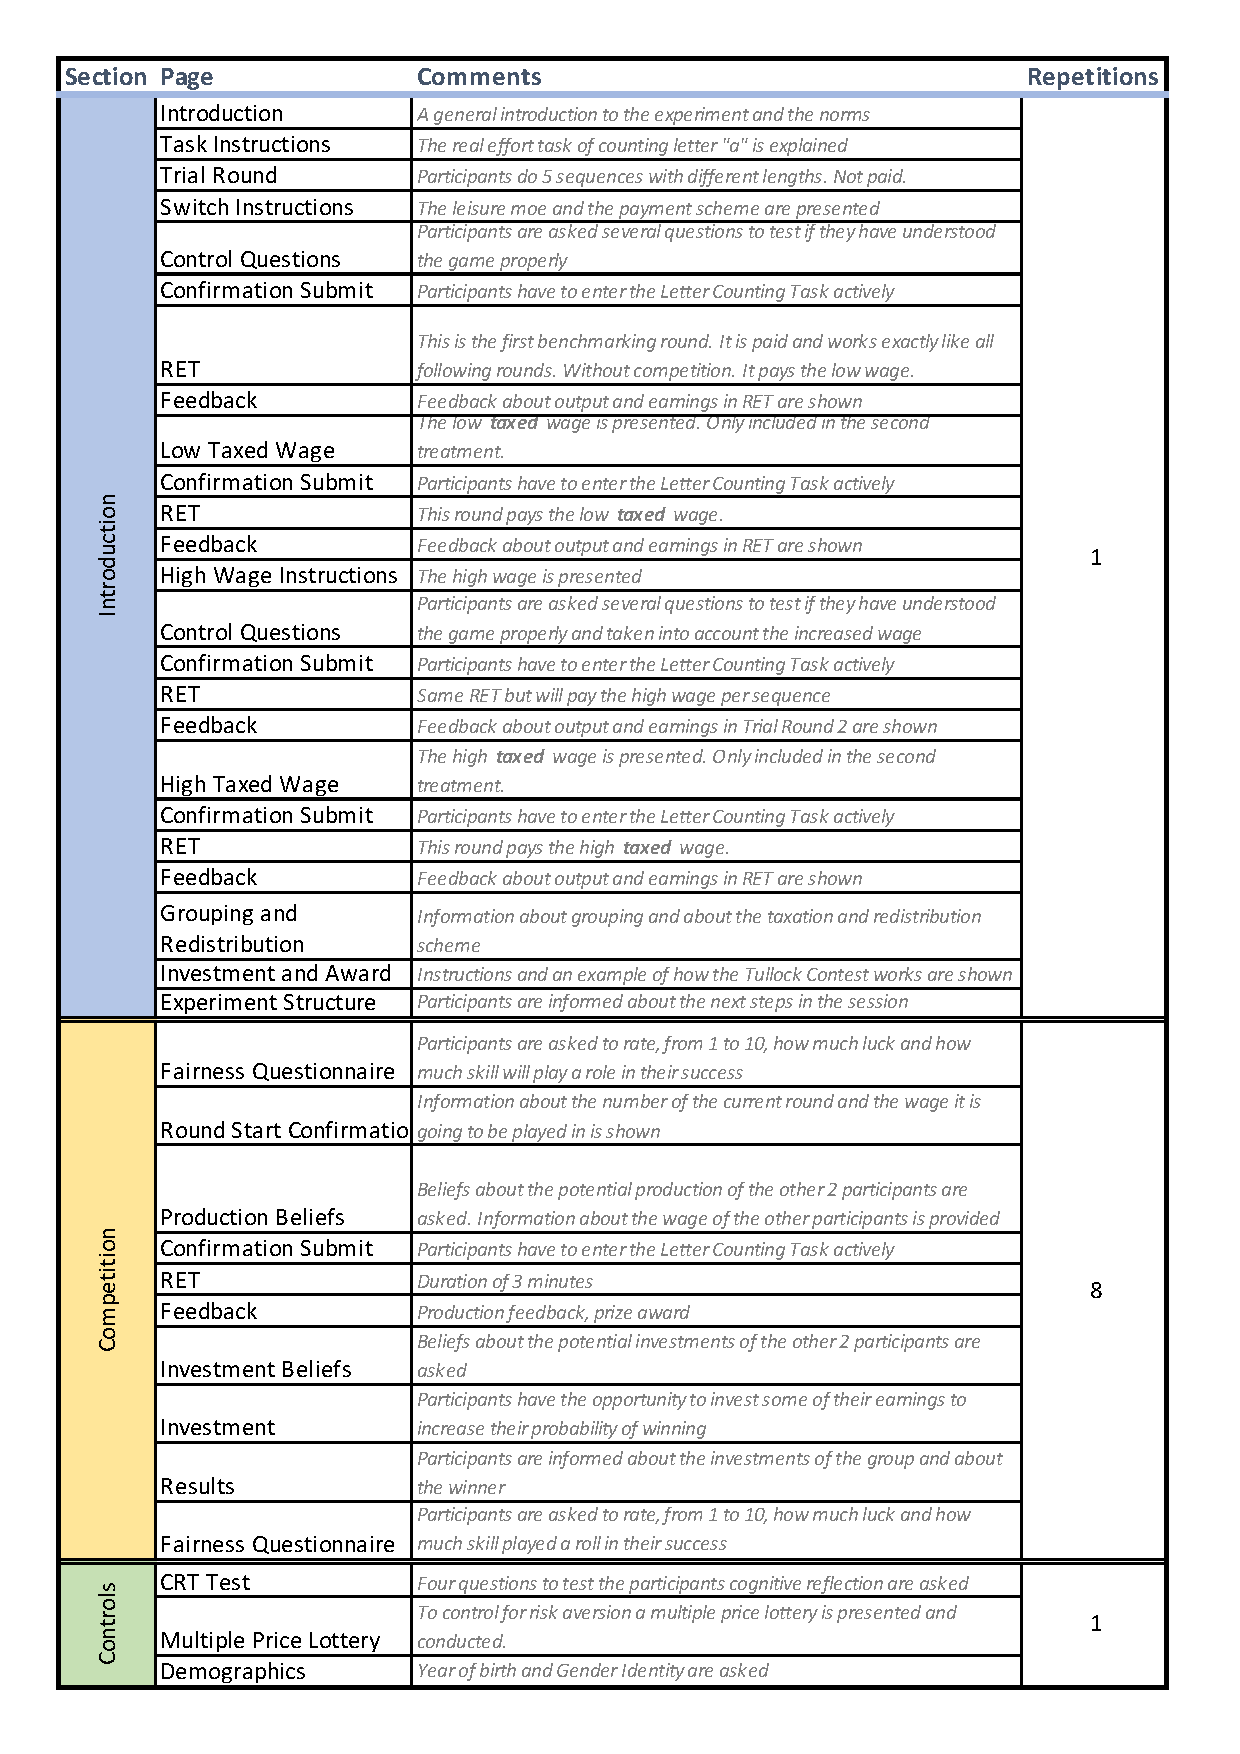
\includegraphics[width=\textwidth]{graphs/Experimental_Design.pdf}
        \caption{Detailed structure of the experiment}
        \label{tab:exp_design}
    \end{figure}
    
\begin{table}[!htbp] \centering 
  \caption{GLMM Probability of Winning} 
  \label{ax:glm_prob} 
\begin{tabular}{@{\extracolsep{5pt}}lc} 
\\[-1.8ex]\hline 
\hline \\[-1.8ex] 
\\[-1.8ex] & \multicolumn{1}{c}{Probability of Winning} \\ 
\\[-1.8ex] & (3)\\ 
\hline \\[-1.8ex] 
 treatment & $-$0.091 \\ 
  & (0.218) \\ 
  &  \\ 
 available income & 0.044$^{***}$  \\ 
  & (0.008) \\ 
  & \\ 
 was winner & $-$0.056 \\ 
  & (0.121) \\ 
  & \\ 
 gender (male) & 0.317\\ 
   & (0.225) \\ 
   & \\ 
 CRT score  & $-$0.036 \\ 
  & (0.113) \\ 
  & \\ 
 risk aversion & 0.036 \\ 
  & (0.049) \\ 
  & \\ 
 valuation & 0.060 \\ 
  & (0.038) \\ 
  & \\ 
 mean investment belief & 0.002 \\ 
  & (0.009) \\ 
  & \\
 cumulative wins & $-$0.037 \\ 
  & (0.028) \\ 
  & \\ 
 Constant & $-$2.364$^{***}$ \\ 
  & (0.650) \\ 
  & \\ 
  \hline
Observations & 672 \\ 
Log Likelihood & 3801.8 \\ 
Akaike Inf. Crit. & $-$7575.6 \\ 
Bayesian Inf. Crit. & $-$7512.5 \\
\hline
Num. groups: participant:group     &   96   \\
Num. groups: group               &    32  \\
Num. groups: round               & 7        \\
\hline
Var: participant:group (Intercept) &  0.872     \\
Var: group (Intercept) &          0.00     \\
Var: round (Intercept)  &          0.00    \\
\hline
\hline \\[-1.8ex] 
\textit{Notes:} & \multicolumn{1}{l}{$^{***}$Significant at the 1 percent level.} \\ 
 & \multicolumn{1}{l}{$^{**}$Significant at the 5 percent level.} \\ 
 & \multicolumn{1}{l}{$^{*}$Significant at the 10 percent level.} \\ 
\end{tabular} 
\end{table} 

\chapter{Screenshots}
\label{ax:screenshots}

\begin{figure}
\centering
\resizebox{1\columnwidth}{!}{%
\begin{tabular}{cc}
\subcaptionbox{Welcome Screen\label{1}}{
\includegraphics[width = 1.5in]{Screenshots/001-174-Welcome.png}} &
\subcaptionbox{Introduction Screen \label{2}}{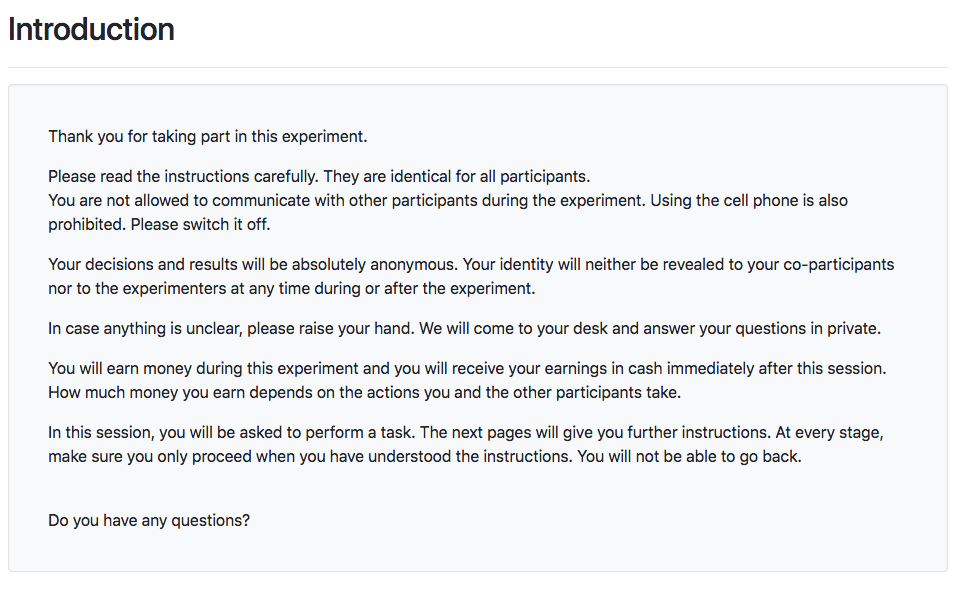
\includegraphics[width = 1.5in]{Screenshots/002-174-Introduction.png}} \\
\subcaptionbox{RET Instructions\label{3}}{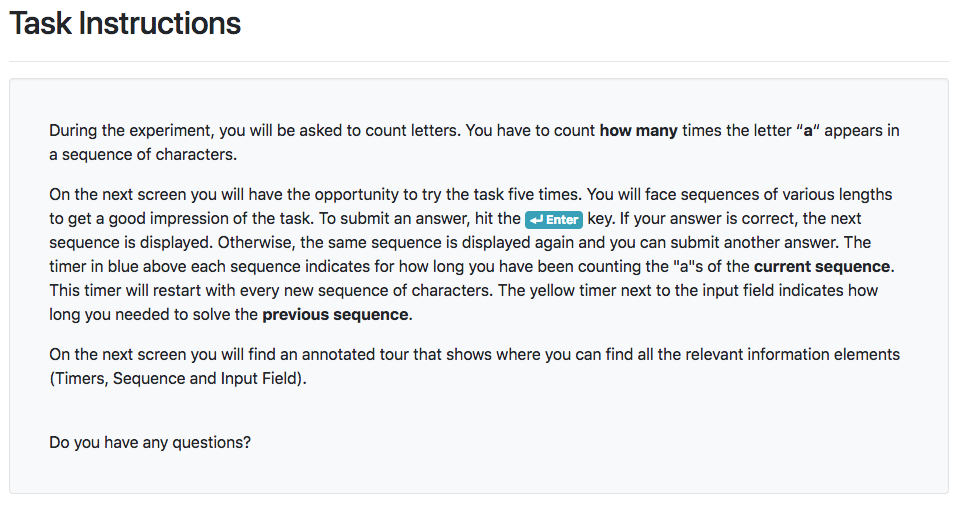
\includegraphics[width = 1.5in]{Screenshots/003-174-Instructions-Trial.png}}&
\subcaptionbox{Test Run Screen\label{4}}{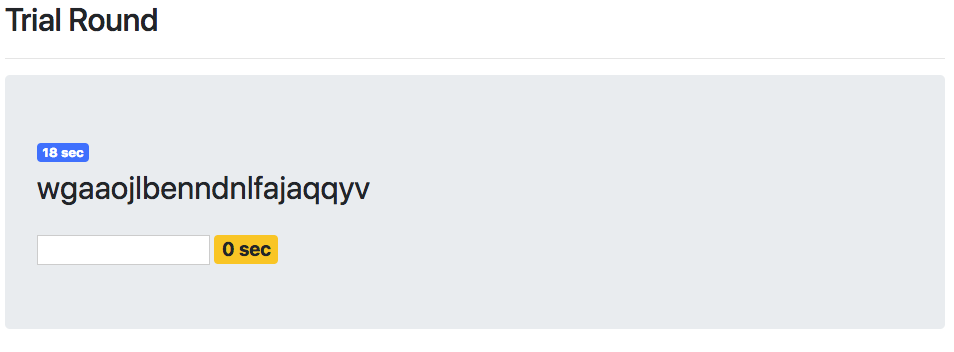
\includegraphics[width = 1.5in]{Screenshots/004-174-Trial-Task.png}} \\
\subcaptionbox{Payment Instructions Screen\label{5}}{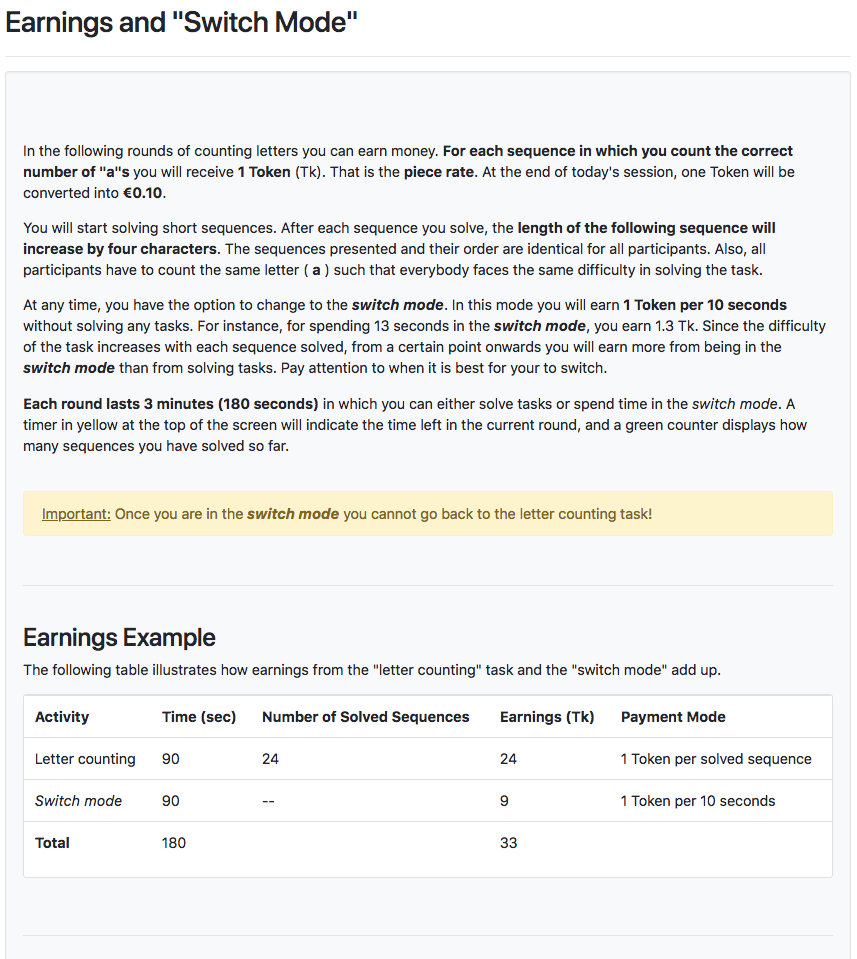
\includegraphics[width = 1.5in]{Screenshots/006-174-Switch_Instructions-1-2.png}} &
\subcaptionbox{Payment Instructions Screen\label{6}}{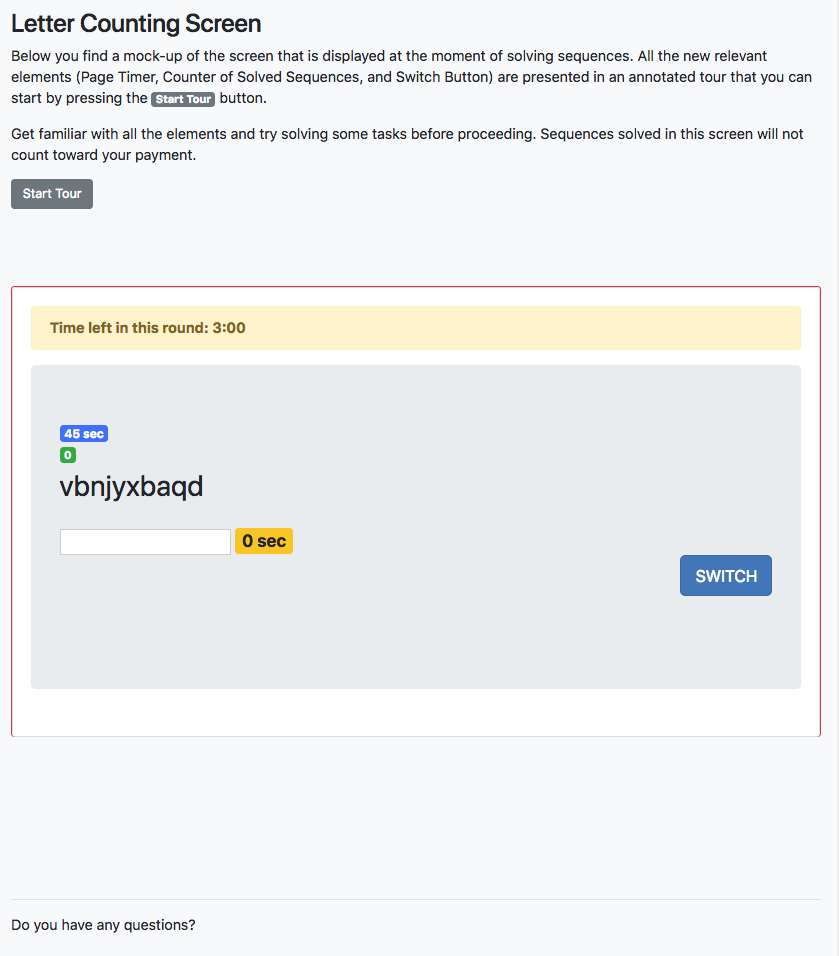
\includegraphics[width = 1.5in]{Screenshots/006-174-Switch_Instructions-2-2.png}}\\
\end{tabular}
}
\caption{Screenshot Selection}
\label{ax:screenshot_1}
\end{figure}

\begin{figure}
\centering
\resizebox{1\columnwidth}{!}{%
\begin{tabular}{ll}
\subcaptionbox{Control Questions\label{7}}{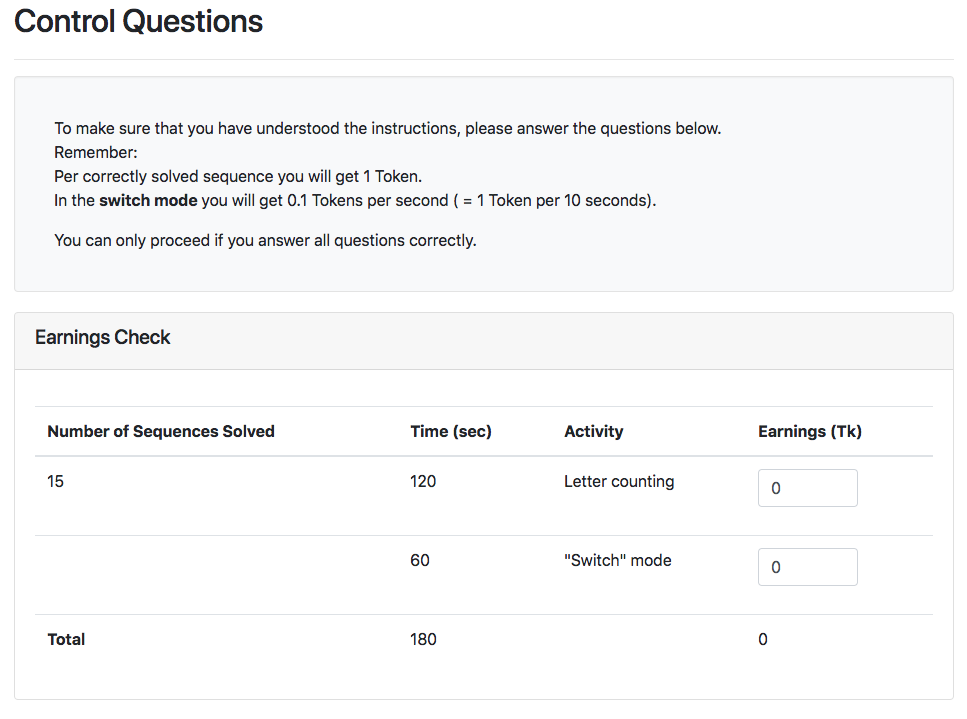
\includegraphics[width = 1.5in]{Screenshots/007-174-Control_Q_Low-1-2.png}} &
\subcaptionbox{Control Questions\label{8}}{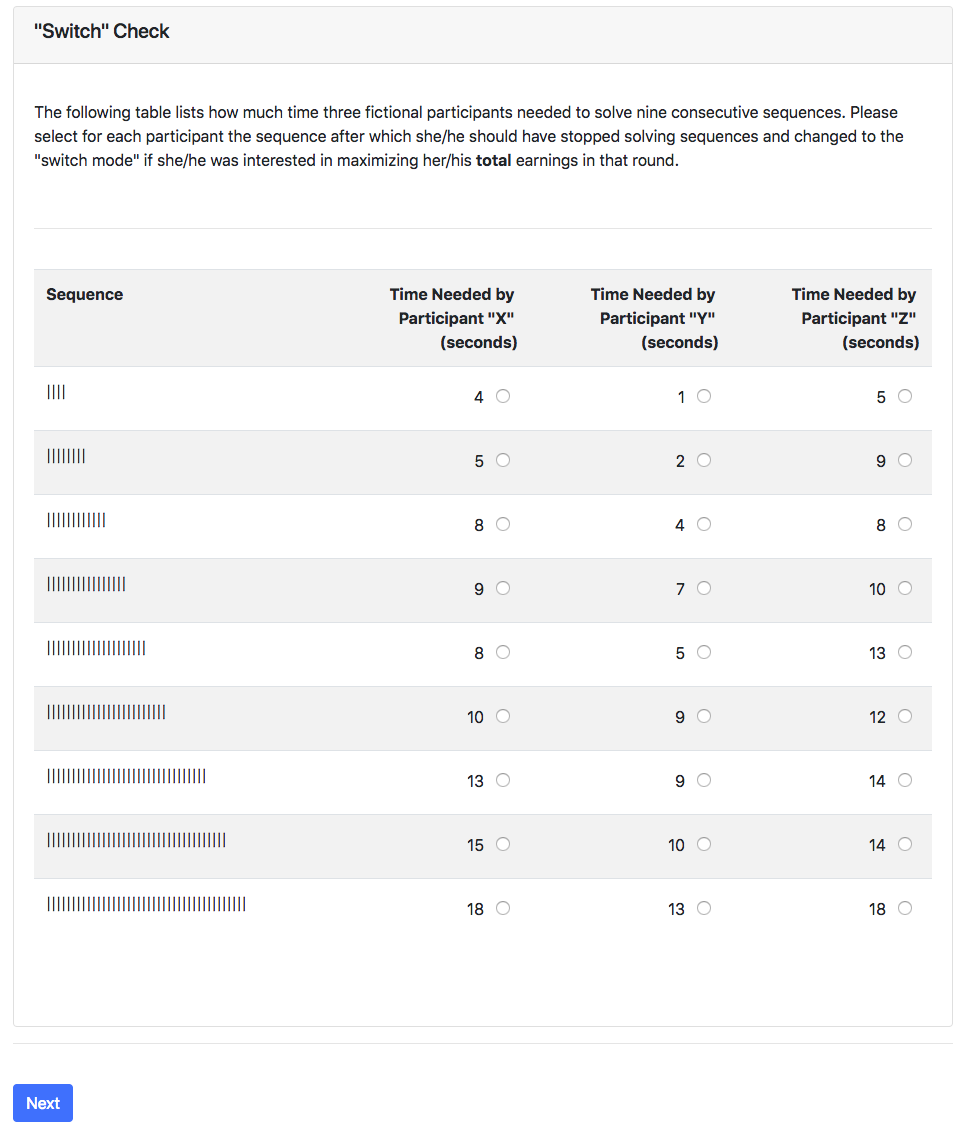
\includegraphics[width = 1.5in]{Screenshots/007-174-Control_Q_Low-2-2.png}} \\
\subcaptionbox{Start of Task Confirmation Screen\label{9}}{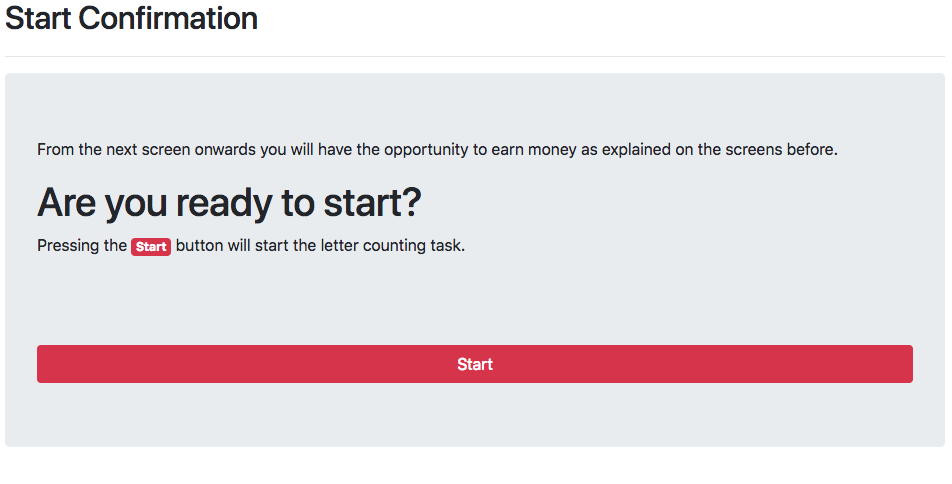
\includegraphics[width = 1.5in]{Screenshots/009-174-Start-RET.png}} &
\subcaptionbox{RET Screen\label{10}}{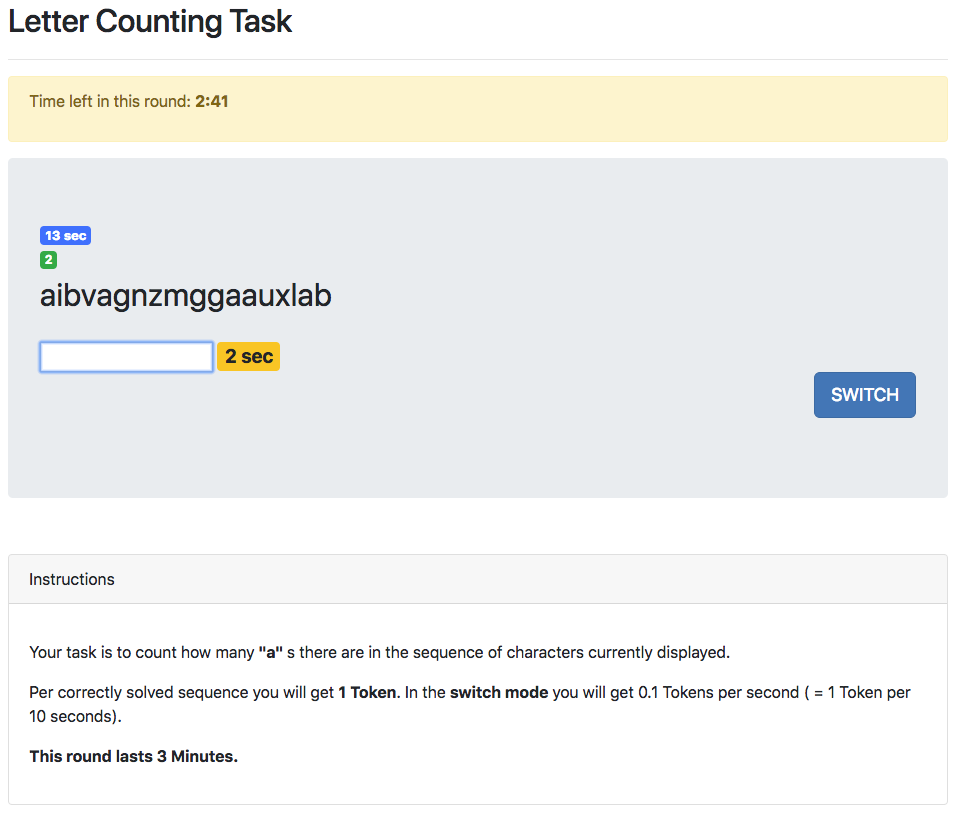
\includegraphics[width = 1.5in]{Screenshots/010-174-RET-1-2.png}} \\
\subcaptionbox{RET Switch Mode\label{11}}{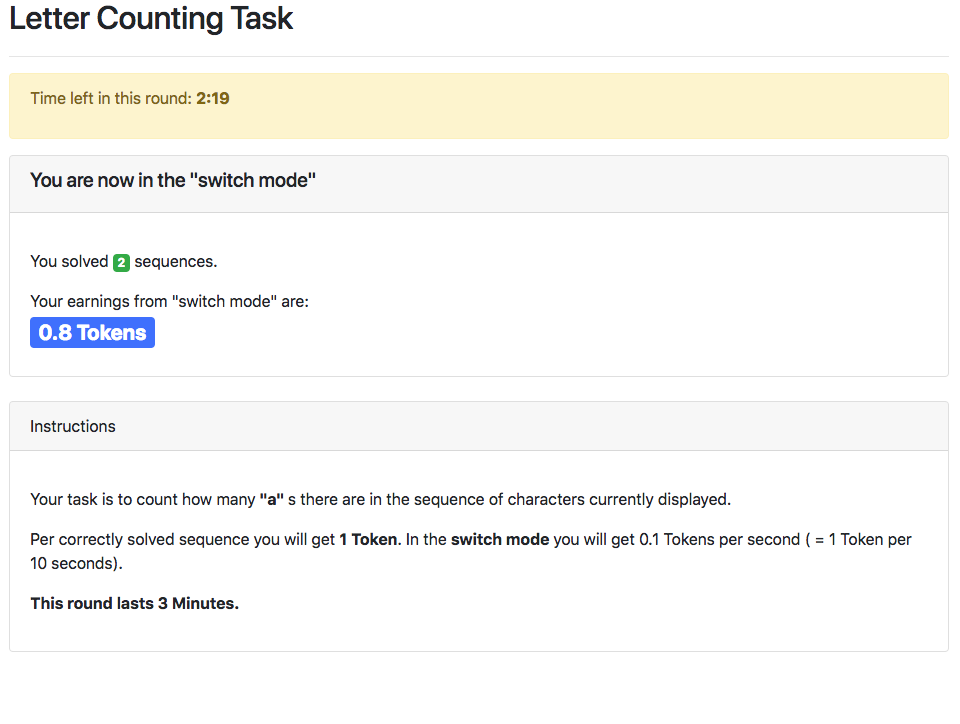
\includegraphics[width = 1.5in]{Screenshots/010-174-RET-2-2.png}} &
\subcaptionbox{RET Feedback Benchmarking\label{12}}{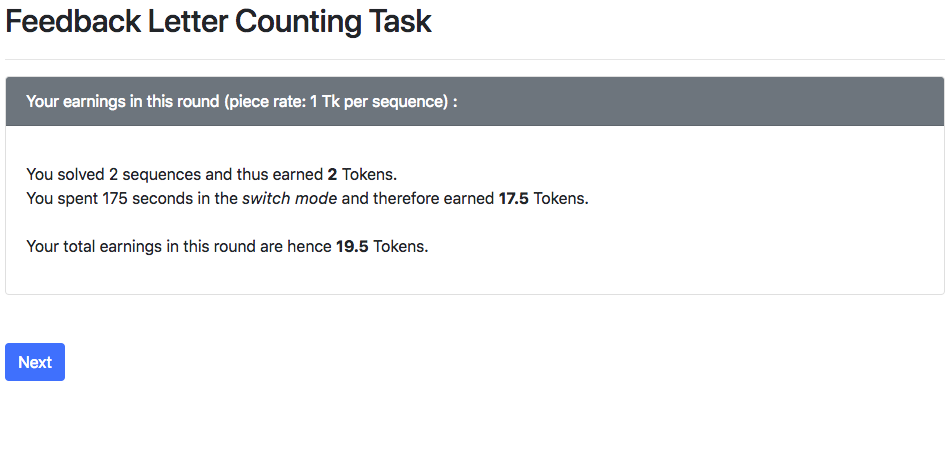
\includegraphics[width = 1.5in]{Screenshots/012-174-Feedback_Low.png}}\\
\end{tabular}
}
\caption{Screenshot Selection}
\label{ax:screenshot_2}
\end{figure}

\begin{figure}
\centering
\resizebox{1\columnwidth}{!}{%
\begin{tabular}{cc}
\subcaptionbox{High Piece Rate Earning Instructions\label{13}}{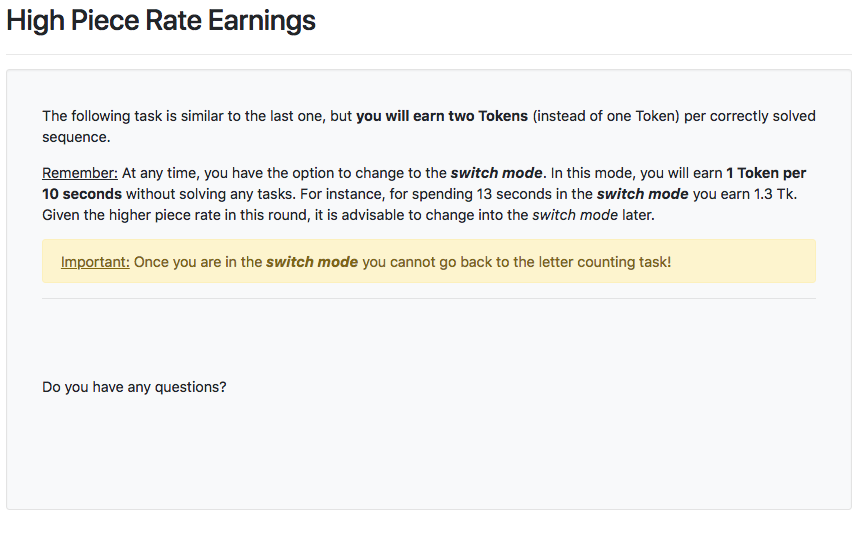
\includegraphics[width = 1.5in]{Screenshots/013-174-High-Instructions.png}} &
\subcaptionbox{Control Questions\label{14}}{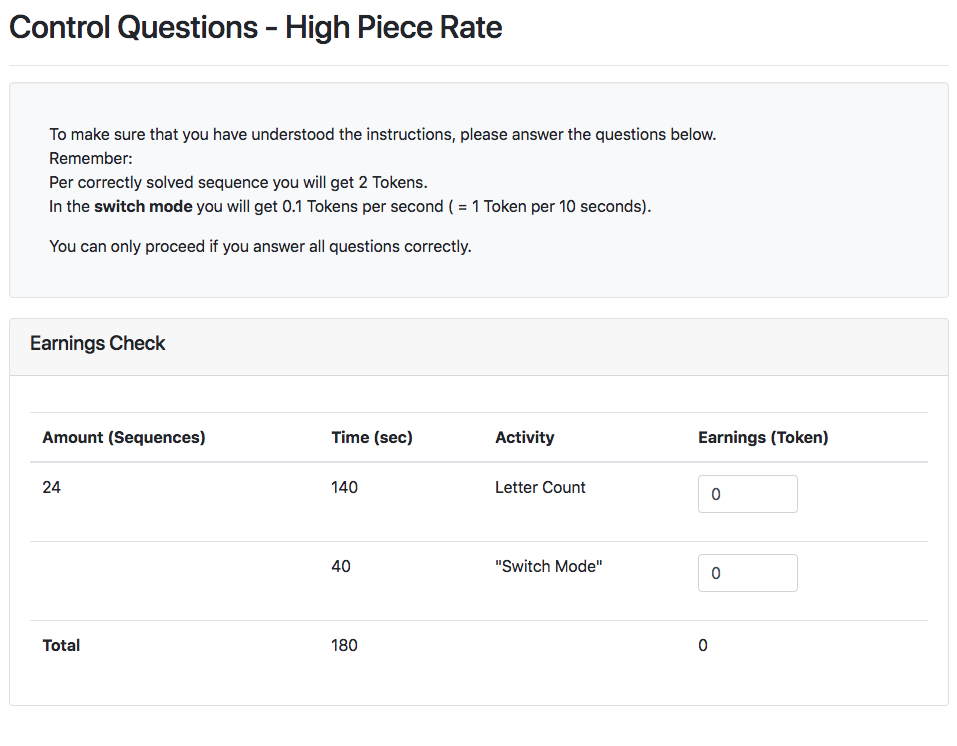
\includegraphics[width = 1.5in]{Screenshots/014-174-Control_Q_High-1-2.png}} \\
\subcaptionbox{Control Questions\label{15}}{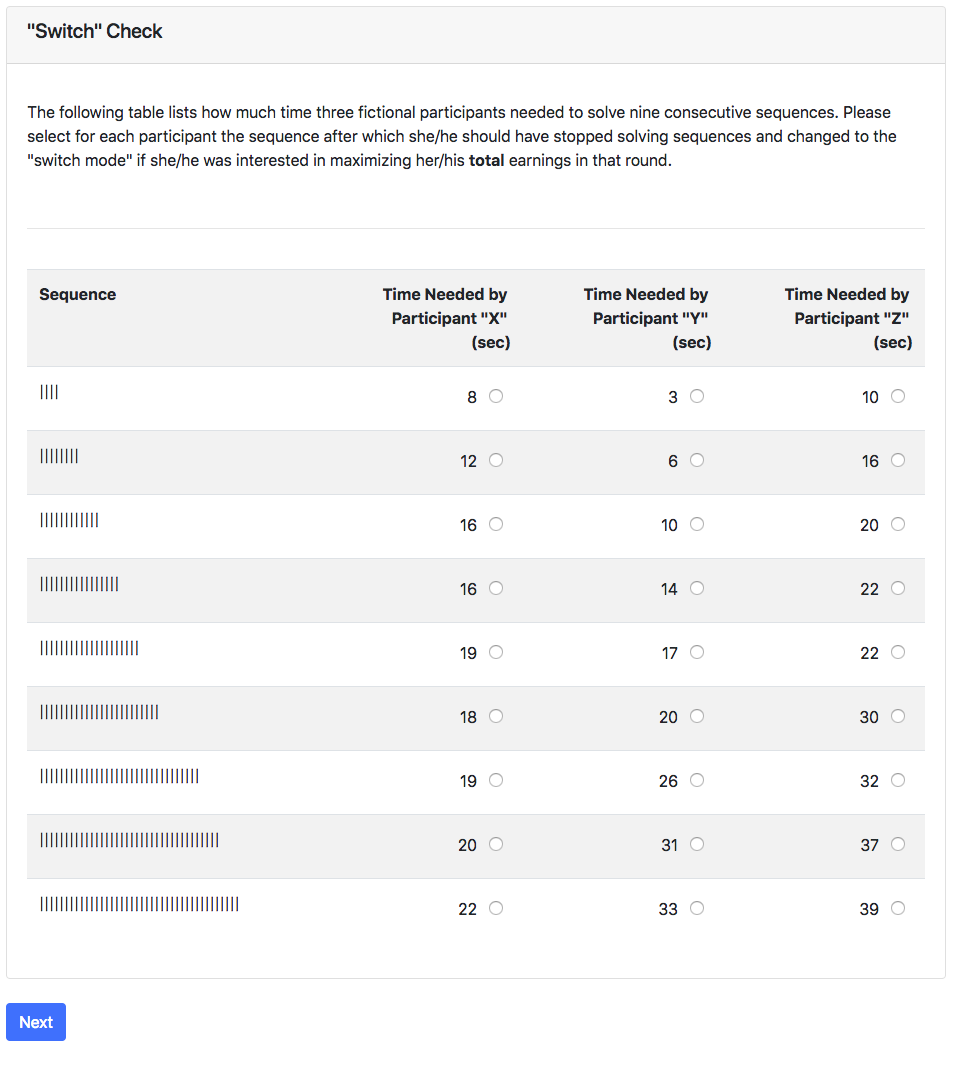
\includegraphics[width = 1.5in]{Screenshots/014-174-Control_Q_High-2-2.png}}&
\subcaptionbox{RET Feedback Benchmarking\label{16}}{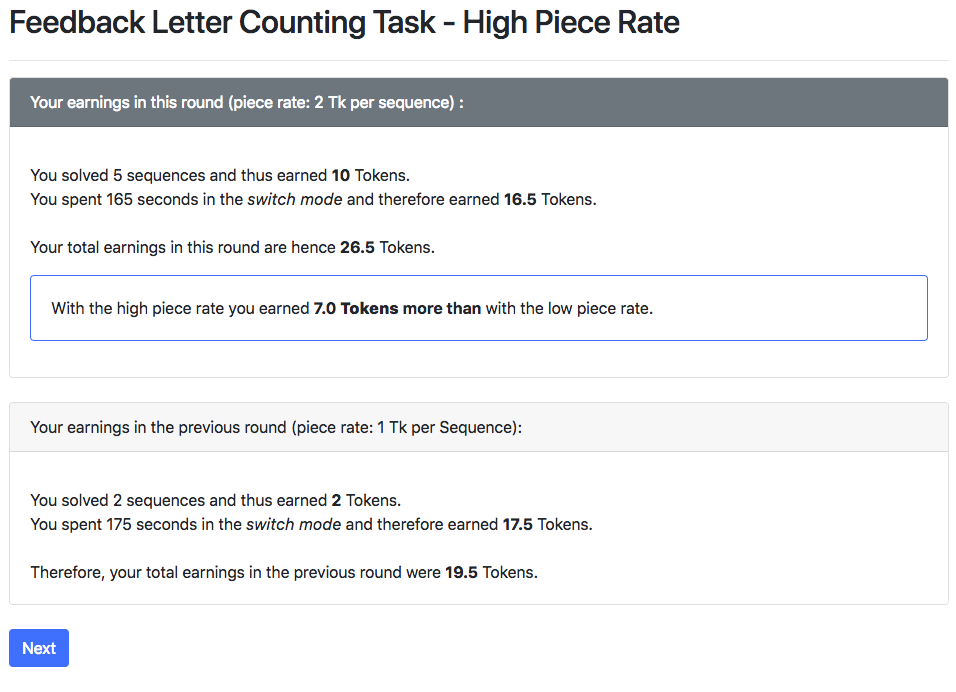
\includegraphics[width = 1.5in]{Screenshots/024-174-Feedback_High.png}} \\
\subcaptionbox{Competition Instructions\label{17}}{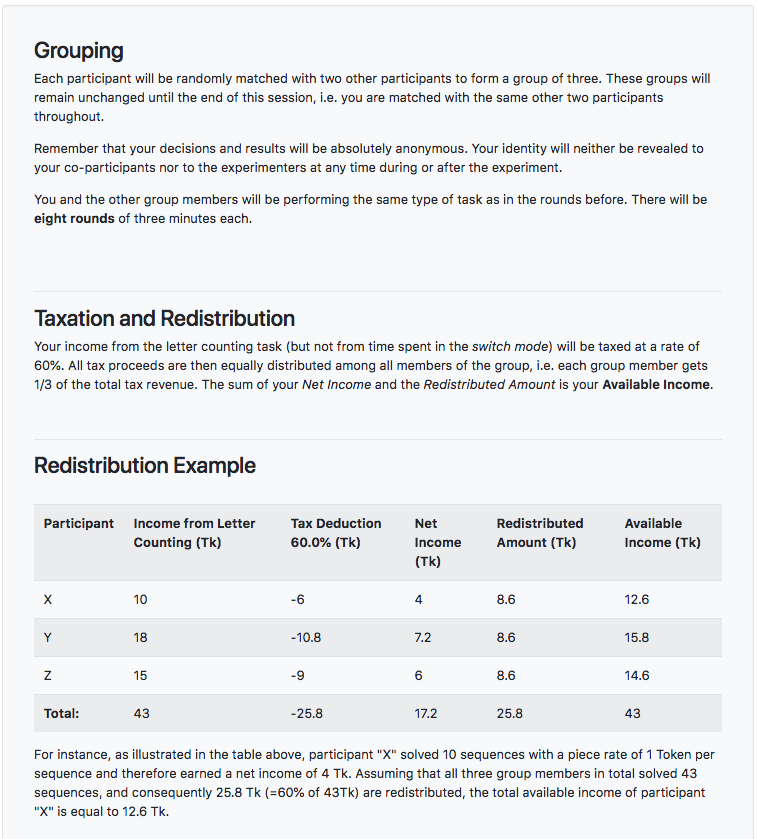
\includegraphics[width = 1.5in]{Screenshots/031-174-Grouping_and_Redi.png}} &
\subcaptionbox{Investment Instructions\label{18}}{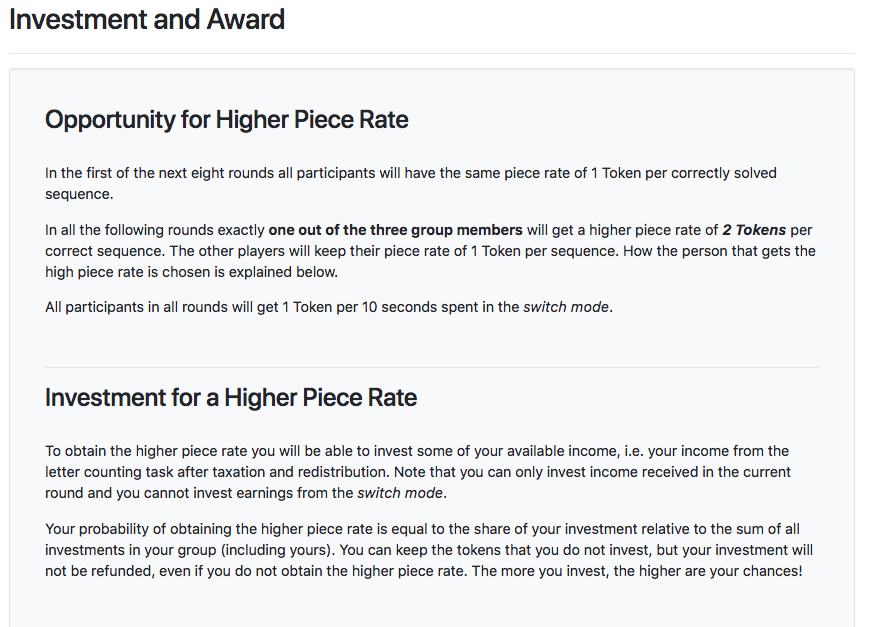
\includegraphics[width = 1.5in]{Screenshots/032-174-Investment_Instructions-1-2.png}}\\
\end{tabular}
}
\caption{Screenshot Selection}
\label{ax:screenshot_3}
\end{figure}

\begin{figure}
\centering
\resizebox{1\columnwidth}{!}{%
\begin{tabular}{cc}
\subcaptionbox{Structure of Experiment Screen\label{19}}{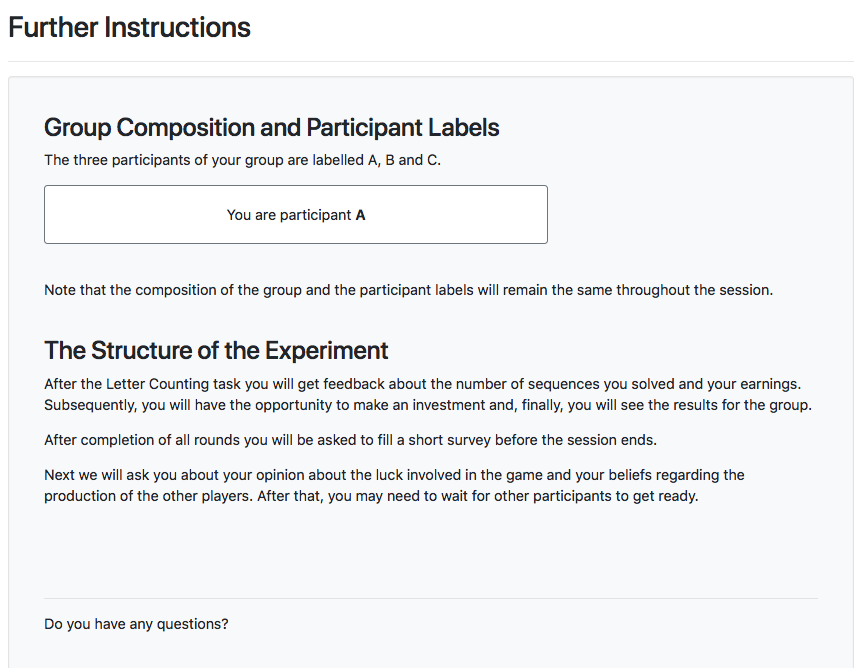
\includegraphics[width = 1.5in]{Screenshots/033-174-Structure.png}} &
\subcaptionbox{Fairness Questionnaire\label{20}}{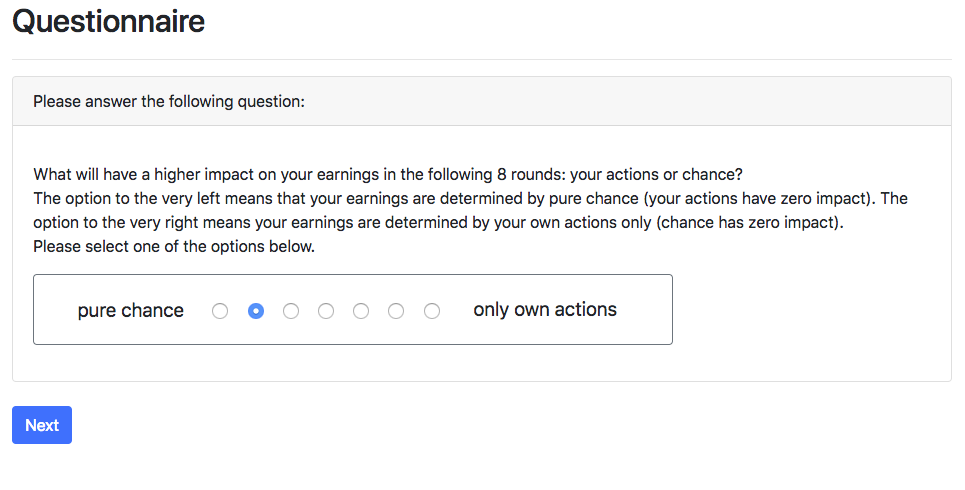
\includegraphics[width = 1.5in]{Screenshots/034-174-Fairness_Q_Begin.png}} \\
\subcaptionbox{Round Marker Screen\label{21}}{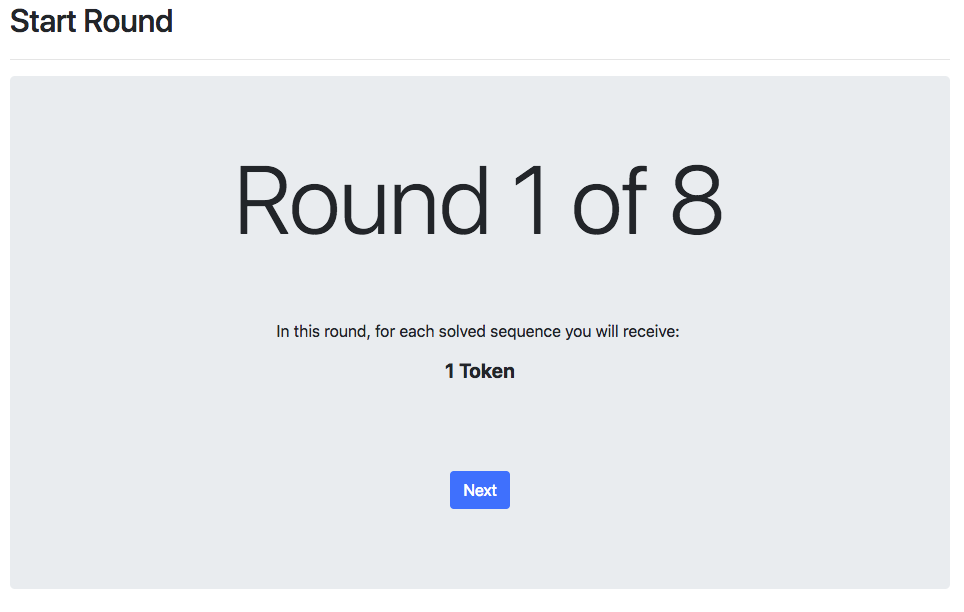
\includegraphics[width = 1.5in]{Screenshots/035-174-RoundStart.png}}&
\subcaptionbox{Production Beliefs Elicitation screen\label{22}}{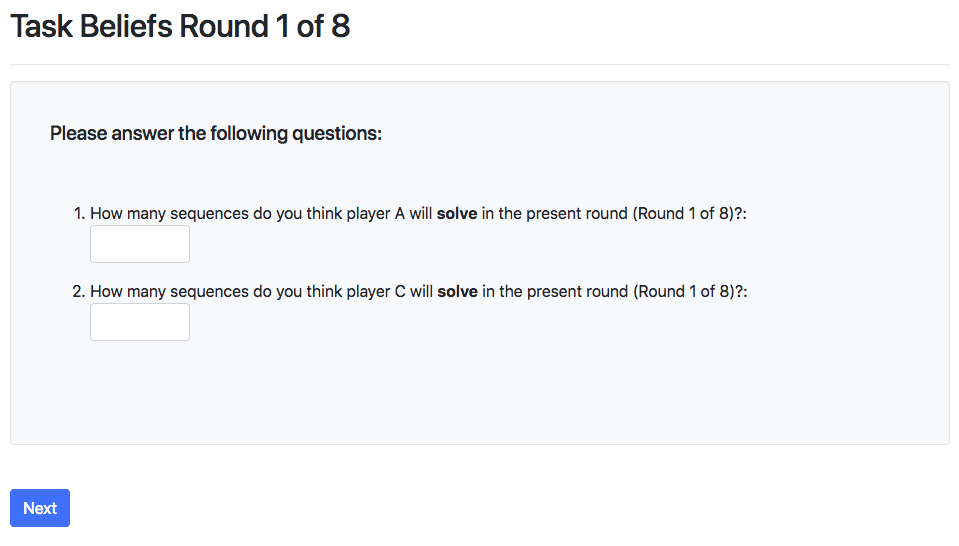
\includegraphics[width = 1.5in]{Screenshots/036-174-Beliefs_Prod.png}} \\
\subcaptionbox{RET Feedback Screen\label{23}}{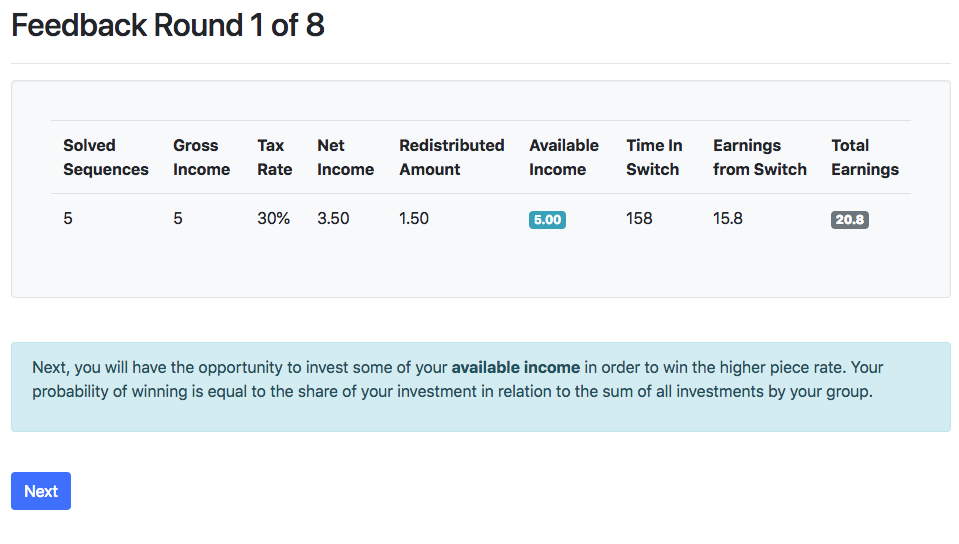
\includegraphics[width = 1.5in]{Screenshots/041-174-Feedback-RET.png}} &
\subcaptionbox{Investment Beliefs Elicitation\label{24}}{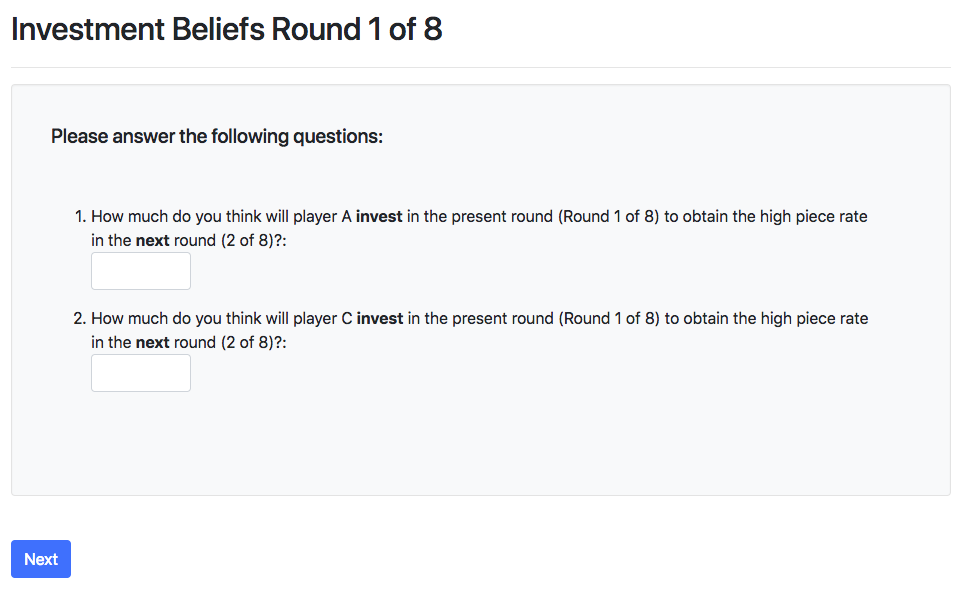
\includegraphics[width = 1.5in]{Screenshots/042-174-Beliefs_Investment.png}}\\
\end{tabular}
}
\caption{Screenshot Selection}
\label{ax:screenshot_4}
\end{figure}


\begin{figure}
\centering
\resizebox{1\columnwidth}{!}{%
\begin{tabular}{cc}
\subcaptionbox{Investment Screen\label{25}}{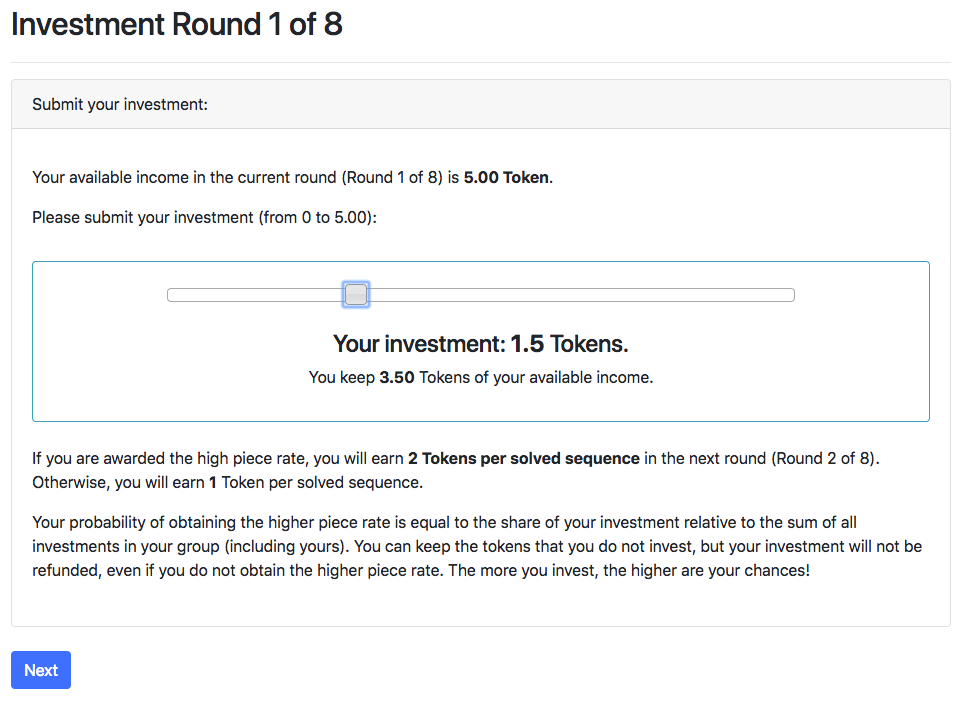
\includegraphics[width = 1.5in]{Screenshots/043-174-Investment.png}} &
\subcaptionbox{Investment Feedback Screen\label{26}}{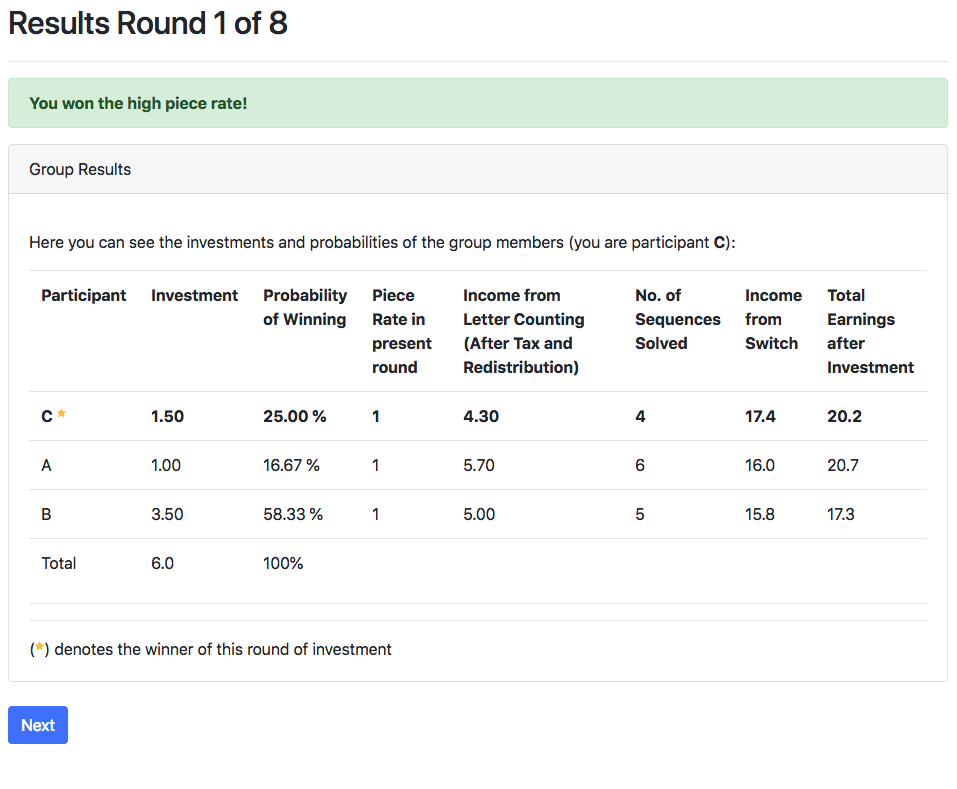
\includegraphics[width = 1.5in]{Screenshots/045_174-Results.png}} \\
\subcaptionbox{Control Questions Marker Screen\label{28}}{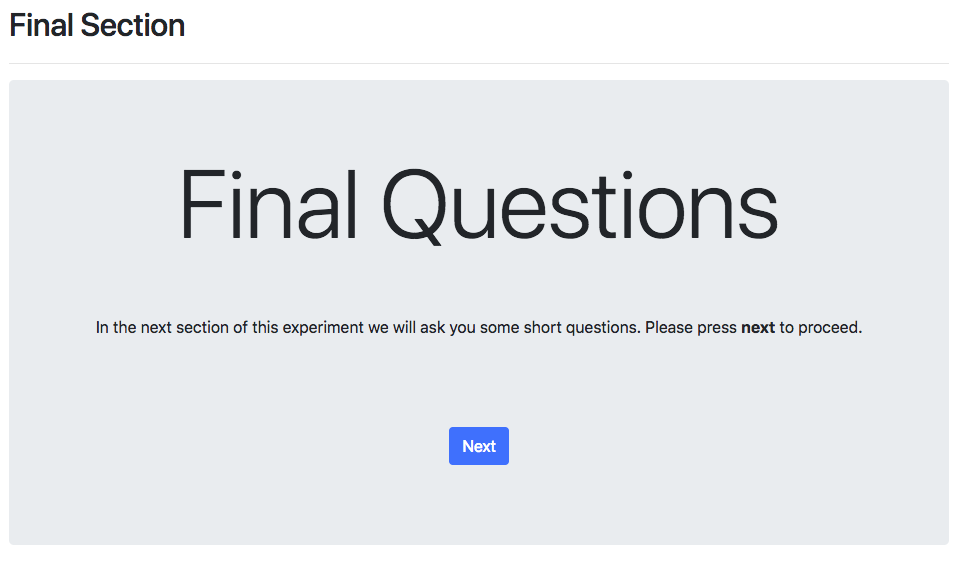
\includegraphics[width = 1.5in]{Screenshots/166-174-Final_Q_Start.png}} &
\subcaptionbox{MLP Instructions\label{33}}{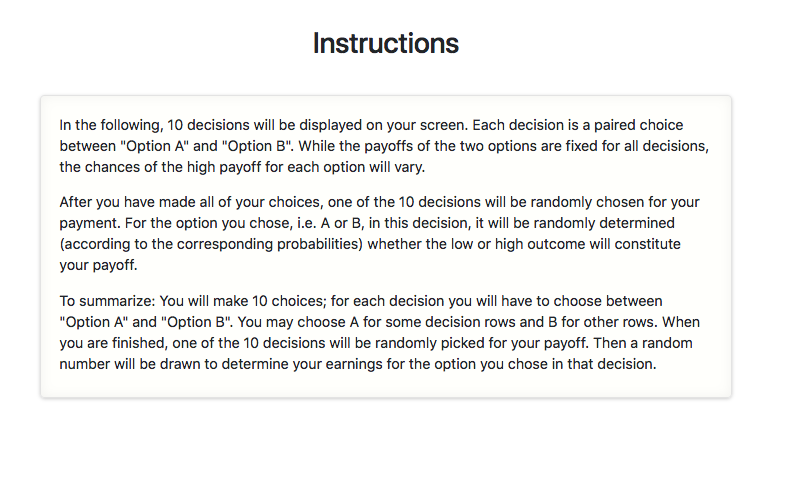
\includegraphics[width = 1.5in]{Screenshots/169-174-Instructions-MPL.png}}\\
\subcaptionbox{MLP Screen\label{34}}{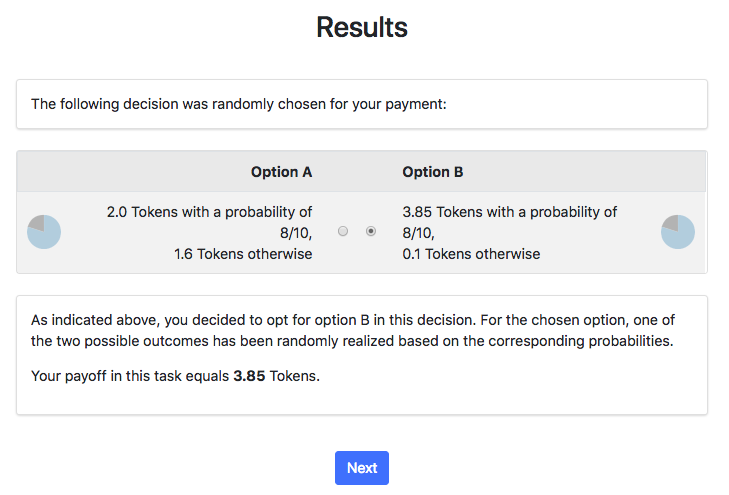
\includegraphics[width = 1.5in]{Screenshots/171-174-Results-MPL.png}} &
\subcaptionbox{Demographics Questionnaire\label{36}}{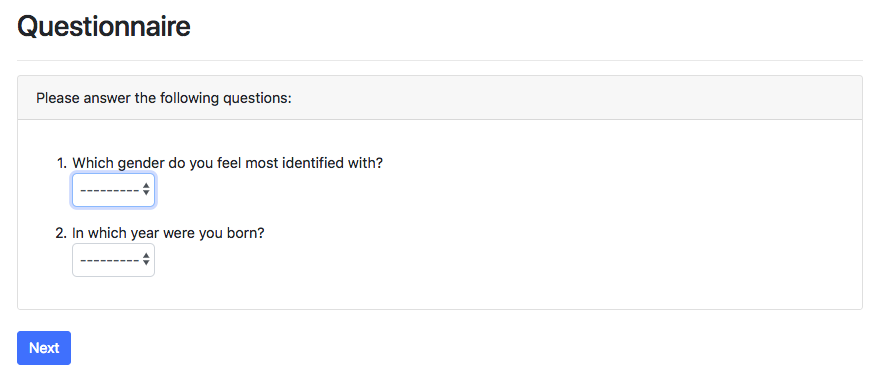
\includegraphics[width = 1.5in]{Screenshots/172-174-Demographics.png}}\\
\end{tabular}
}
\caption{Screenshot Selection}
\label{ax:screenshot_5}
\end{figure}



\end{appendices}